\section{Activities}\label{sec:activities}

There are many activities to be considered that are important for the completion of this project. As we are working on potentially safety-critical software, we need to have a thorough understanding of the requirements and a solid design to base our implementation on. To ensure that the requirements specification matches the actual needs of our customers and that our software design and architecture supports the correct implementation of these requirements, we will continuously update and refine the requirements and the design. Another important part of our project is the quality assurance process which helps us check our own work constantly throughout the project.

\subsection{Technical feasibility analysis}\label{sec:feasibility}

As the Åboat software project is already implemented as a microservice architecture, we are sure that the VRGP implementation will be able to run within the existing software environment of the Åboat. Basically, it means adding another microservice - as a Docker container - which runs the vessel-side VRGP implementation and communicates with the other microservices, especially those that provide the sensor data of the Åboat. No, or very minimal, additional hardware, which would be provided by the Åboat project, needs to be added to support the VRGP implementation on the Åboat.
\\\\
A minimal proof of concept for the VRGP protocol also already exists in the form of a simple MOC test implementation (available on \href{https://github.com/RemoteBoatX/vrgp-docs/tree/main/moc-environment}{GitHub}) which communicates with a mobile device, simulating a vessel in this context. The mobile device can transmit very basic information: network time, response latency, and basic video output. This prototype implementation is by AboaMare.

\subsection{Requirement analysis}\label{sec:requirements}

In the initial phase of the project, we will be in regular and close contact to our customers to acquire a thorough understanding of the requirements and to formulate these initial requirements as the basic pillar for the design of the system. These requirements will be continuously reassessed and refined over the course of the project.
\\\\
We agreed with our customers to split the system into a maximum of ten high-level functional requirements which will be refined by sub-requirements. This ensures that the requirements can be easily understood even by persons not familiar with the technicalities of the project. It also lays a foundation for the design of the software.
\\\\
The requirements can be found and will be updated and refined in the technical documentation of this project.

\subsection{Design}\label{sec:design}

The software design and architecture will be based on the requirements, as described in the previous section. Like the requirements, the design will be reassessed and refined throughout the project. While the requirements are to be negotiated closely coordinated with the customers, most of the software design and architecture within the given software environment are up to us. The boundaries that are set by the existing software environment are:

\begin{itemize}
	\item The VRGP implementation for the Åboat runs as a microservice or a set of microservices within a microservice architecture.
	\item The microservice is deployed as an independent Docker container.
	\item The microservice communicates with other microservices within the Åboat software environment.
	\item The existing MOC test implementation by AboaMare can serve partly as a guide for our MOC prototype.
\end{itemize}

\subsection{Implementation}\label{sec:implementation}

Following the initial design phase and based on the software design and architecture, we will begin implementing the actual system. It will probably mostly be implementation challenges and realisation during this phase, that make reassessment of the existing requirements and design necessary.
\\\\
As there are already systems present on the Åboat that we need to interface with, we have an initial technology stack already in place, which we have to build upon. This consists of the following technologies already present:

\begin{itemize}
	\item OpenDLV (main framework for communication between microservices)
	\item C++ as a server and interfacing language
	\item Docker as a container solution
	\item JavaScript was used to build the existing prototype for the Maritime Operating Center
\end{itemize}

\noindent
We might need or want to use additional technologies to facilitate our implementation, to test the existing and new code, to integrate on the already existing system, or to communicate with other systems already in place. These might include tools like:

\begin{itemize}
	\item Zabbix (for monitoring)
	\item Postman (for API testing and interaction)
	\item Additional languages for easier prototyping (Python)
\end{itemize}

\noindent
The implementation of the system can be split into the following major tasks, which might be extended over the course of the project:

\begin{itemize}
	\item Developing the software in an independent container capable of interacting with the other parts of the system.
	\item Creating the necessary network and communication infrastructure.
	\item Implementing the vessel side of the VRGP protocol.
	\item Testing the communication between a mock-up MOC and the vessel.
\end{itemize}

\subsection{Quality assurance}\label{sec:quality}

Over the course of the project, beginning with the initial requirements analysis phase, we will have quality assurance measures in place to ensure a safe and high-quality software product. An important part of this process will be the regular meetings with our customers as well as peer and team reviews within our project team.
\\\\
With the beginning of the implementation phase, we will conduct software quality checks with every feature added or piece of code changed. This includes:

\begin{itemize}
	\item Continuous testing and integration
	\item Continuous deployment and application building
	\item Security checks
	\item Quality assurance of the final product
\end{itemize}

\noindent
This way there will be a continuous tracking of the product quality. Throughout the project, we will also make sure that the features which are being developed respect the requirements agreed upon with the customers. If any requirements change, we will adapt the software accordingly.
\\\\
Following the prototyping phase of the project, we will also use monitoring tools to ensure the proper functioning of both the server and the client-side software.

\section{Tasks, milestones and schedule}\label{sec:schedule}

The schedule is rather detailed by now, but is reevaluated and adjusted every week in our team meetings. The planned phases, especially those that lie further in the future, are estimated and subject to change over the course of the project.

\begin{figure}[ht]
	\centering
	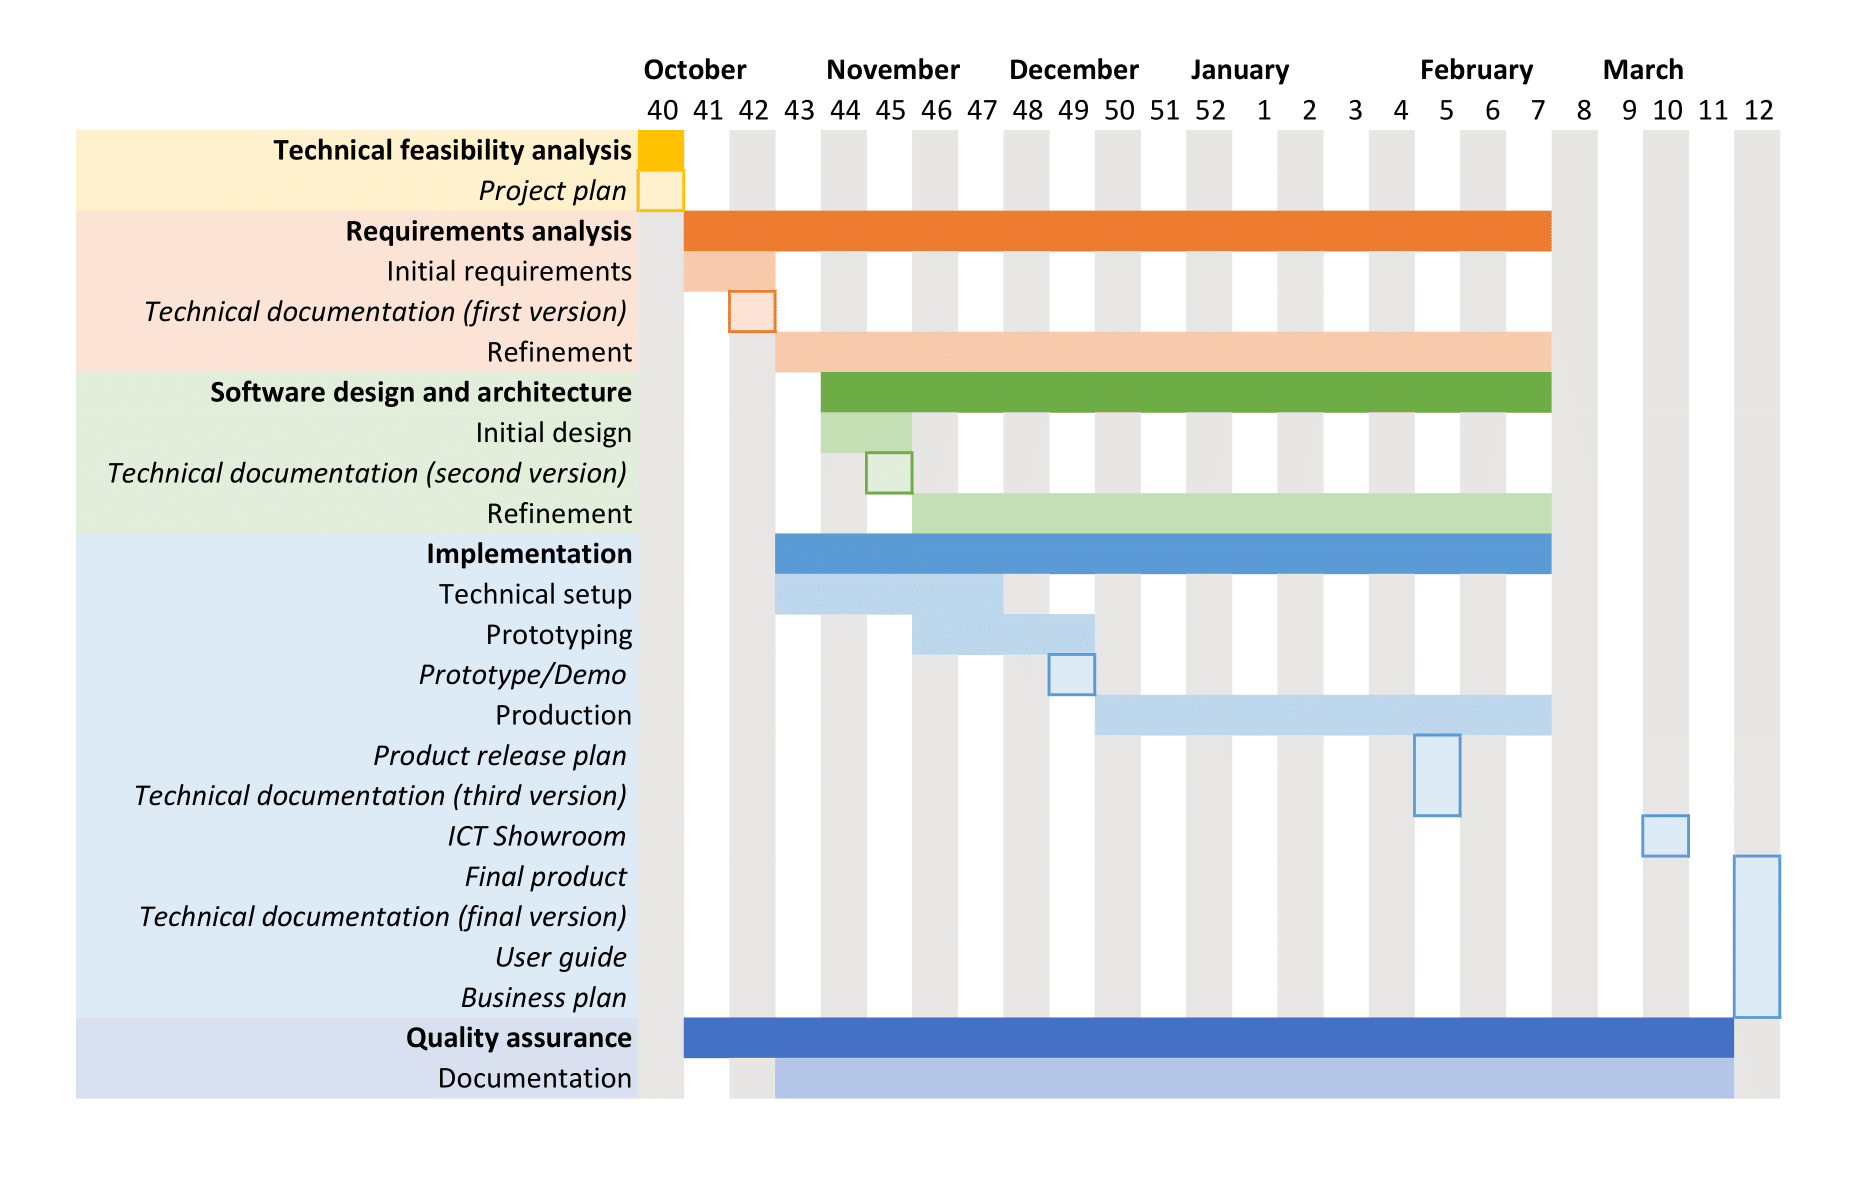
\includegraphics[width=\linewidth]{img/schedule}
	\caption{Schedule}
	\label{fig:schedule}
\end{figure}
